\documentclass[final, slidestop]{beamer}

\title{Mutalyzer 2.0: Improved sequence variant descriptions from \\
  next generation sequencing data and gene variant databases}
\author{Jeroen F.J. Laros, Martijn Vermaat, Gerben Stouten, 
  Johan T. den Dunnen, Peter E.M. Taschner}
\institute{Center for Human and Clinical Genetics, Leiden University Medical
  Center, Leiden, The Netherlands}
\providecommand{\centerLogo}{
  \includegraphics[height = 3cm]{gen2phen_logo}
}
\providecommand{\rightLogo}{
  \includegraphics[height = 3cm]{nbic_logo}
}
\providecommand{\colOneWidth}{0.48}
\providecommand{\colTwoWidth}{0.48}

\usetheme{lumc}

\begin{document}

\begin{frame}{}
  \begin{myPoster}
    \colorBlock{Background}{Introduction}{1}{
      Unambiguous and correct sequence variant descriptions are of utmost
      importance for DNA diagnostics. The free Mutalyzer sequence variation
      nomenclature checker 
      (\color{red}\bt{http://www.mutalyzer.nl/}\color{LUMCBlue}) names variants
      following the Human Genome Variation Society (HGVS) sequence variant
      nomenclature recommendations~\cite{HGVS}.

      \begin{figure}
        \vspace{2cm}
        \setlength{\unitlength}{0.12cm}
        \vspace{-0.5cm}
\begin{center}
  \colorbox{white}{
    \begin{picture}(300, 60)(0, 0)
      \put(0, 30){\line(1, 0){300}}  % Genomic sequence.
      \linethickness{4pt}
      \put(50, 30){\line(1, 0){30}}  % Non-coding parts of the exons.
      \put(220, 30){\line(1, 0){10}}
      \linethickness{12pt}
      \put(80, 30){\line(1, 0){20}}  % Coding parts of the exons.
      \put(150, 30){\line(1, 0){20}}
      \put(200, 30){\line(1, 0){20}}

      \linethickness{0.5pt}
      \put(20, 50){\scriptsize{Transcription start}}
      \put(50, 45){\vector(0, -1){10}}
      \put(200, 50){\scriptsize{Transcription end}}
      \put(230, 45){\vector(0, -1){10}}

      \put(70, 0){\scriptsize{CDS start}}
      \put(80, 10){\vector(0, 1){10}}
      \put(210, 0){\scriptsize{CDS stop}}
      \put(220, 10){\vector(0, 1){10}}

      \put(0, 0){\scriptsize{Genomic end}}
      \put(0, 10){\vector(0, 1){10}}
      \put(270, 0){\scriptsize{Genomic start}}
      \put(300, 10){\vector(0, 1){10}}

      \put(95, 50){\color{red}\scriptsize{Variant A}\color{black}}
      \put(115, 45){\color{red}\vector(0, -1){10}\color{black}}

      \put(140, 50){\color{red}\scriptsize{Variant B}\color{black}}
      \put(160, 45){\color{red}\vector(0, -1){10}\color{black}}
    \end{picture}
  }
\end{center}
\bigskip

        \caption{Gene-centred key positions in HGVS numbering scheme.}
        \label{fig:positions}
      \end{figure}

      \begin{table}
        \caption{HGVS positions in genomic (g.), non-coding (n.) and coding DNA
          (c.) notations.}
        \colorbox{white}{
        {\small
          \begin{tabular}{l|r|r|r}
            Key position        & \bt{g.}  & \bt{n.}      & \bt{c.} \\
            \hline
            Genomic start       & \bt{1}    & \bt{1-u470}   & \bt{-29-u470} \\
            Transcription start & \bt{471}  & \bt{1}        & \bt{-29} \\
            CDS start           & \bt{501}  & \bt{30}       & \bt{1} \\
            Intron 1 start      & \bt{513}  & \bt{41+1}     & \bt{12+1} \\
            Intron 1 end        & \bt{612}  & \bt{42-1}     & \bt{13-1} \\
            CDS stop            & \bt{1830} & \bt{359}      & \bt{330} \\
            Transcription end   & \bt{2050} & \bt{579}      & \bt{*220} \\
            Genomic end         & \bt{2670} & \bt{579+d620} & \bt{*220+d620} \\
          \end{tabular}
          }
        }
      \end{table}
    }
    \colorBlock{WhiteBg}{Conclusions}{1}{
      Variants at intergenic, exonic, intronic, CDS and UTR positions can be
      easily distinguished based on their gene-centered HGVS descriptions.
      Mutalyzer facilitates batch-wise conversion from dbSNP rsIDs or
      chromosomal position numbering of next generation sequencing data to
      transcript position numbering, as well as sequence variant checking of
      locus-specific sequence variant databases (LSDBs)~\cite{LOVD}.
    }
    \colorBlock{SalmonBg}{Position Conversion}{1}{
      The position converter in batch mode is especially suited for NGS
      applications. It can handle large numbers of genomic variant descriptions
      and converts them to transcript-oriented positions. Following a semantic
      check with the batch Name Checker, variant descriptions can be used for
      annotation. CDS, exon and intron positions can be easily distinguished
      from the HGVS descriptions and used to query LSDBs.

      \begin{figure}
        {
          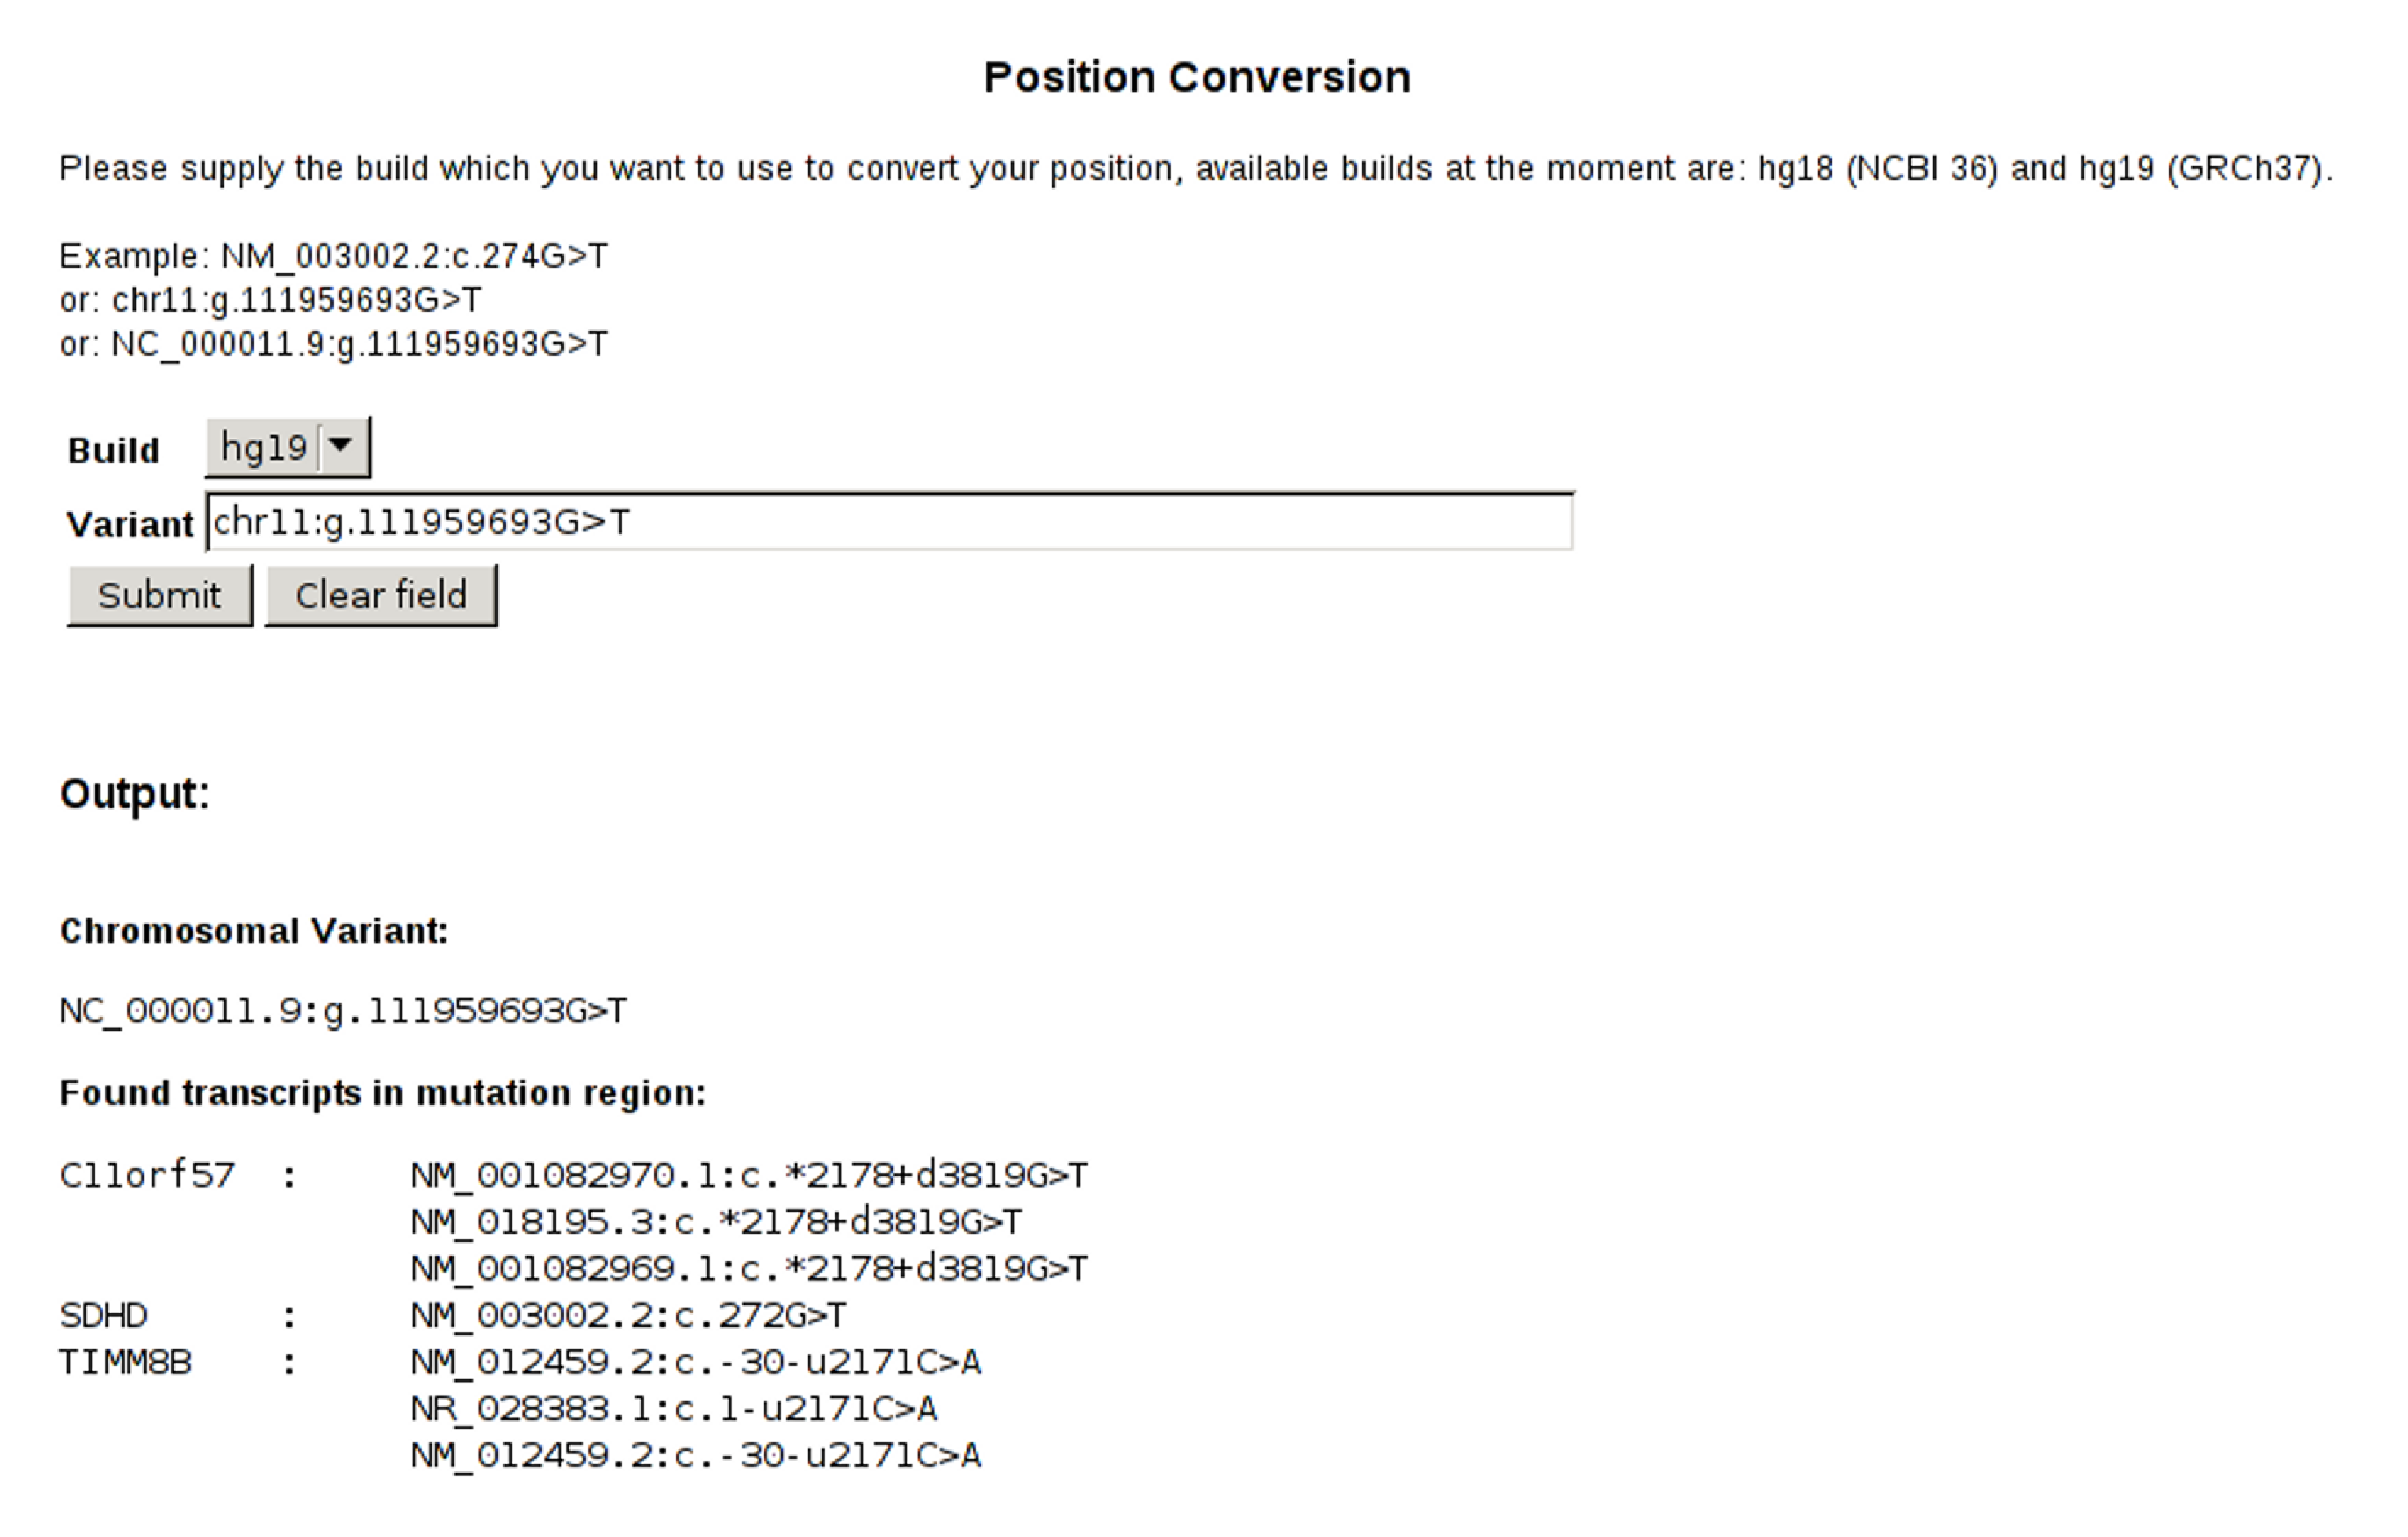
\includegraphics[width = 0.85\textwidth, height = 18cm]{mutalyzerPositionConvert}
        }
        \caption{Mutalyzer 2.0 Position Converter.}
        \label{figure:positionconvert}
      \end{figure}
    }
    \colorBlock{YellowBg}{Acknowledgements}{1}{
      {\small
        Funded by the European Community's Seventh Framework Programme
        (FP7/2007-2013) under grant agreement no. 200754 - the GEN2PHEN project.
      }

    }
    \nextColumn
    \colorBlock{BlueBg}{Name Checking}{1}{
      \begin{figure}
        {
          \includegraphics[width = 0.95\textwidth, height = 57cm]{mutalyzerNameCheck}
        }
        \caption{Mutalyzer 2.0 Name Checker results using the CDKN2A LRG
          reference sequence~\cite{LRG}}
        \label{figure:namecheck}
      \end{figure}
    }
    \colorBlock{GreenBg}{Interfaces}{1}{
      
      \begin{tabular}{l@{\ \ --\ \ }p{25cm}}
        Name Checker       & Syntactic and semantic checks.$^*$
                               (Fig.~\ref{figure:namecheck}) \\
        Syntax Checker     & Syntactic checks only.$^*$ \\
        Position Converter & Convert chromosomal positions to gene-centered
                               notation (no semantic check)$^*$
                               (Fig.~\ref{figure:positionconvert}) \\
        SNP Converter      & Convert a dbSNP rsId to HGVS notation.$^*$ \\
        Name Generator     & Contruct a HGVS notation. \\
        GenBank Uploader   & Upload custom GenBank files. \\
        Webservices        & Programmatic (SOAP) interface. \\
      \end{tabular}
      \bigskip

      $^*$ {\small Also available as a batch interface.}
    }
    \colorBlock{Background}{References}{1}{
      {\small
        \bibliography{$HOME/projects/bibliography}{}
      }
    }
  \end{myPoster}
\end{frame}
\end{document}
